\documentclass[a4paper]{article}
\usepackage[utf8]{inputenc}
\usepackage[russian]{babel}
\usepackage[T2]{fontenc}
\usepackage[warn]{mathtext}
\usepackage{graphicx}
\usepackage{amsmath}
\usepackage{floatflt}
\usepackage{amssymb}
\usepackage[left=20mm, top=20mm, right=20mm, bottom=20mm, footskip=10mm]{geometry}


\graphicspath{ {images/} }
\usepackage{multicol}
\setlength{\columnsep}{2cm}


\begin{document}

\begin{titlepage}
	\centering
	\vspace{5cm}
	{\scshape\LARGE Московский физико-технический институт \par}
	\vspace{4cm}
	{\scshape\Large Лабораторная работа \par}
	\vspace{1cm}
	{\huge\bfseries Изучение спектра водорода \par}
	\vspace{1cm}
	\vfill
\begin{flushright}
	{\large выполнила студентка 653 группы ФФКЭ}\par
	\vspace{0.3cm}
	{\LARGE Карпова Татьяна} \par

\end{flushright}
	

	\vfill

% Bottom of the page
	Долгопрудный, 2018 г.
\end{titlepage}


\section{Цель работы}
\begin{enumerate}
    \item Исследование спектральных закономерностей в оптическом спектре водорода
    \item Вычисление постоянной Ридберга для водорода по результатам измерения
    \item Определение потенциала ионизации водорода
\end{enumerate}

\section{В работе используются}
\begin{itemize}
    \item стеклянно-призменный монохроматор-спектрометр УМ-2
    \item ртутная лампа ПРК-4 для градуировки 
    \item водородная лампа
    \item фотоаппарат для регистрации спектров
\end{itemize}

\section{Теоретические положения}
Длины волн спектральных линий водородоподобного атома описываются формулой
\begin{equation}
    \frac{1}{\lambda_m_n} = RZ^2(\frac{1}{n^2} - \frac{1}{m^2}),
\end{equation}
где $R$ - постоянная Ридберга, а $m, n$ -  целые числа. \par
Использование постулатов Бора с учётом кулоновского взаимодействия между ядром и электроном позволяет легко определить возможные энергетические состояния водородоподобного атома. Если считать ядро неподвижным, то эти энергетические состояния определяются выражением
\begin{equation}
    E_n = -\frac{2 \pi^2 m_e e^4 Z^2}{h^2} \frac{1}{n^2}
\end{equation}

\begin{figure}[h]
    \centering
    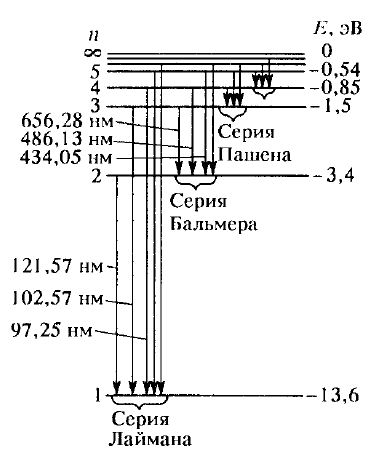
\includegraphics[width=6cm]{fig3.PNG}
    \caption{Уровни энергии атома водорода и образование спектральных серий}
    \label{fig:vac}
\end{figure}

Знание энергетических состояний атома позволяет в соответствии с формулой (2) определить возможные частоты его излучения и объяснить наблюдаемые закономерности. \par
В данной работе изучается серия Бальмера, линии которой лежат в видимой области, и изотопический сдвиг между линиями водорода. Для серии Бальмера в формуле (1) $n = 2$. Величина $m$ для первых четырёх линий этой серии принимает значение 3, 4, 5, 6. \par
Боровский радиус (радиус первой орбиты) для электрона в поле ядра с зарядом $Z$:
\begin{equation}
    r_B = \frac{\hbar^2}{Z m_e e^2}
\end{equation}
Энергия основного состояния:
\begin{equation}
    E = -\frac{m_e e^4}{2 \hbar^2}Z^2 = -R Z^2
\end{equation}
Аналогичным образом могут быть найдены энергии возбуждённых состояний. Дискретные значения энергии электрона в атоме получаются из того условия, что на длине орбиты, по которой движется электрон, должно укладываться целое число волн де Бройля. Если радиус орбиты равен $r$, то $n$-му состоянию электрона соответствует условие 
\begin{equation}
    2 \pi r = \lambda n (n \in \mathbb{N}) ; m_e v_n = \frac{nh}{2 \pi r}
\end{equation}

Аналогично пп. (3)-(4):
\begin{equation}
     r_B = \frac{n^2 \hbar^2}{Z m_e e^2}
\end{equation}

\begin{equation}
    E = -\frac{m_e e^4}{2 \hbar^2} \frac{1}{n^2} Z^2 = -R \frac{Z^2}{n^2}
\end{equation}

\section{Экспериментальная установка}
Для измерения длин волн спектральных линий в работе используется стеклянно-призменный монохроматор-спектрометр УМ-2, предназначенный для спектральных исследований в диапазоне от 0,38 до 1 мкм

\begin{figure}[h]
    \centering
    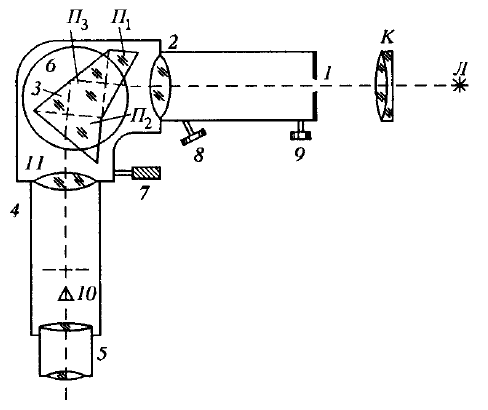
\includegraphics[width=10cm]{fig2.PNG}
    \caption{Устройство монохроматора УМ-12}
    \label{fig:vac}
\end{figure}

Спектрометр нуждается в дополнительной градуировке, проводящейся по спектру ртутной лампы с известными длинами волн спектральных линий.

\section{Выполнение работы}
\begin{enumerate}
    \item Проградуируем спектрометр с помощью программного обеспечения, используя ртутную лампу. Используя "Атлас линий ртути" определим длины волн видимых в спектре линий. Представим спектр на рис. 1, на рис. 2 представлена фотография спектра ртутной лампы.
    
    \begin{figure}[h]
    \centering
    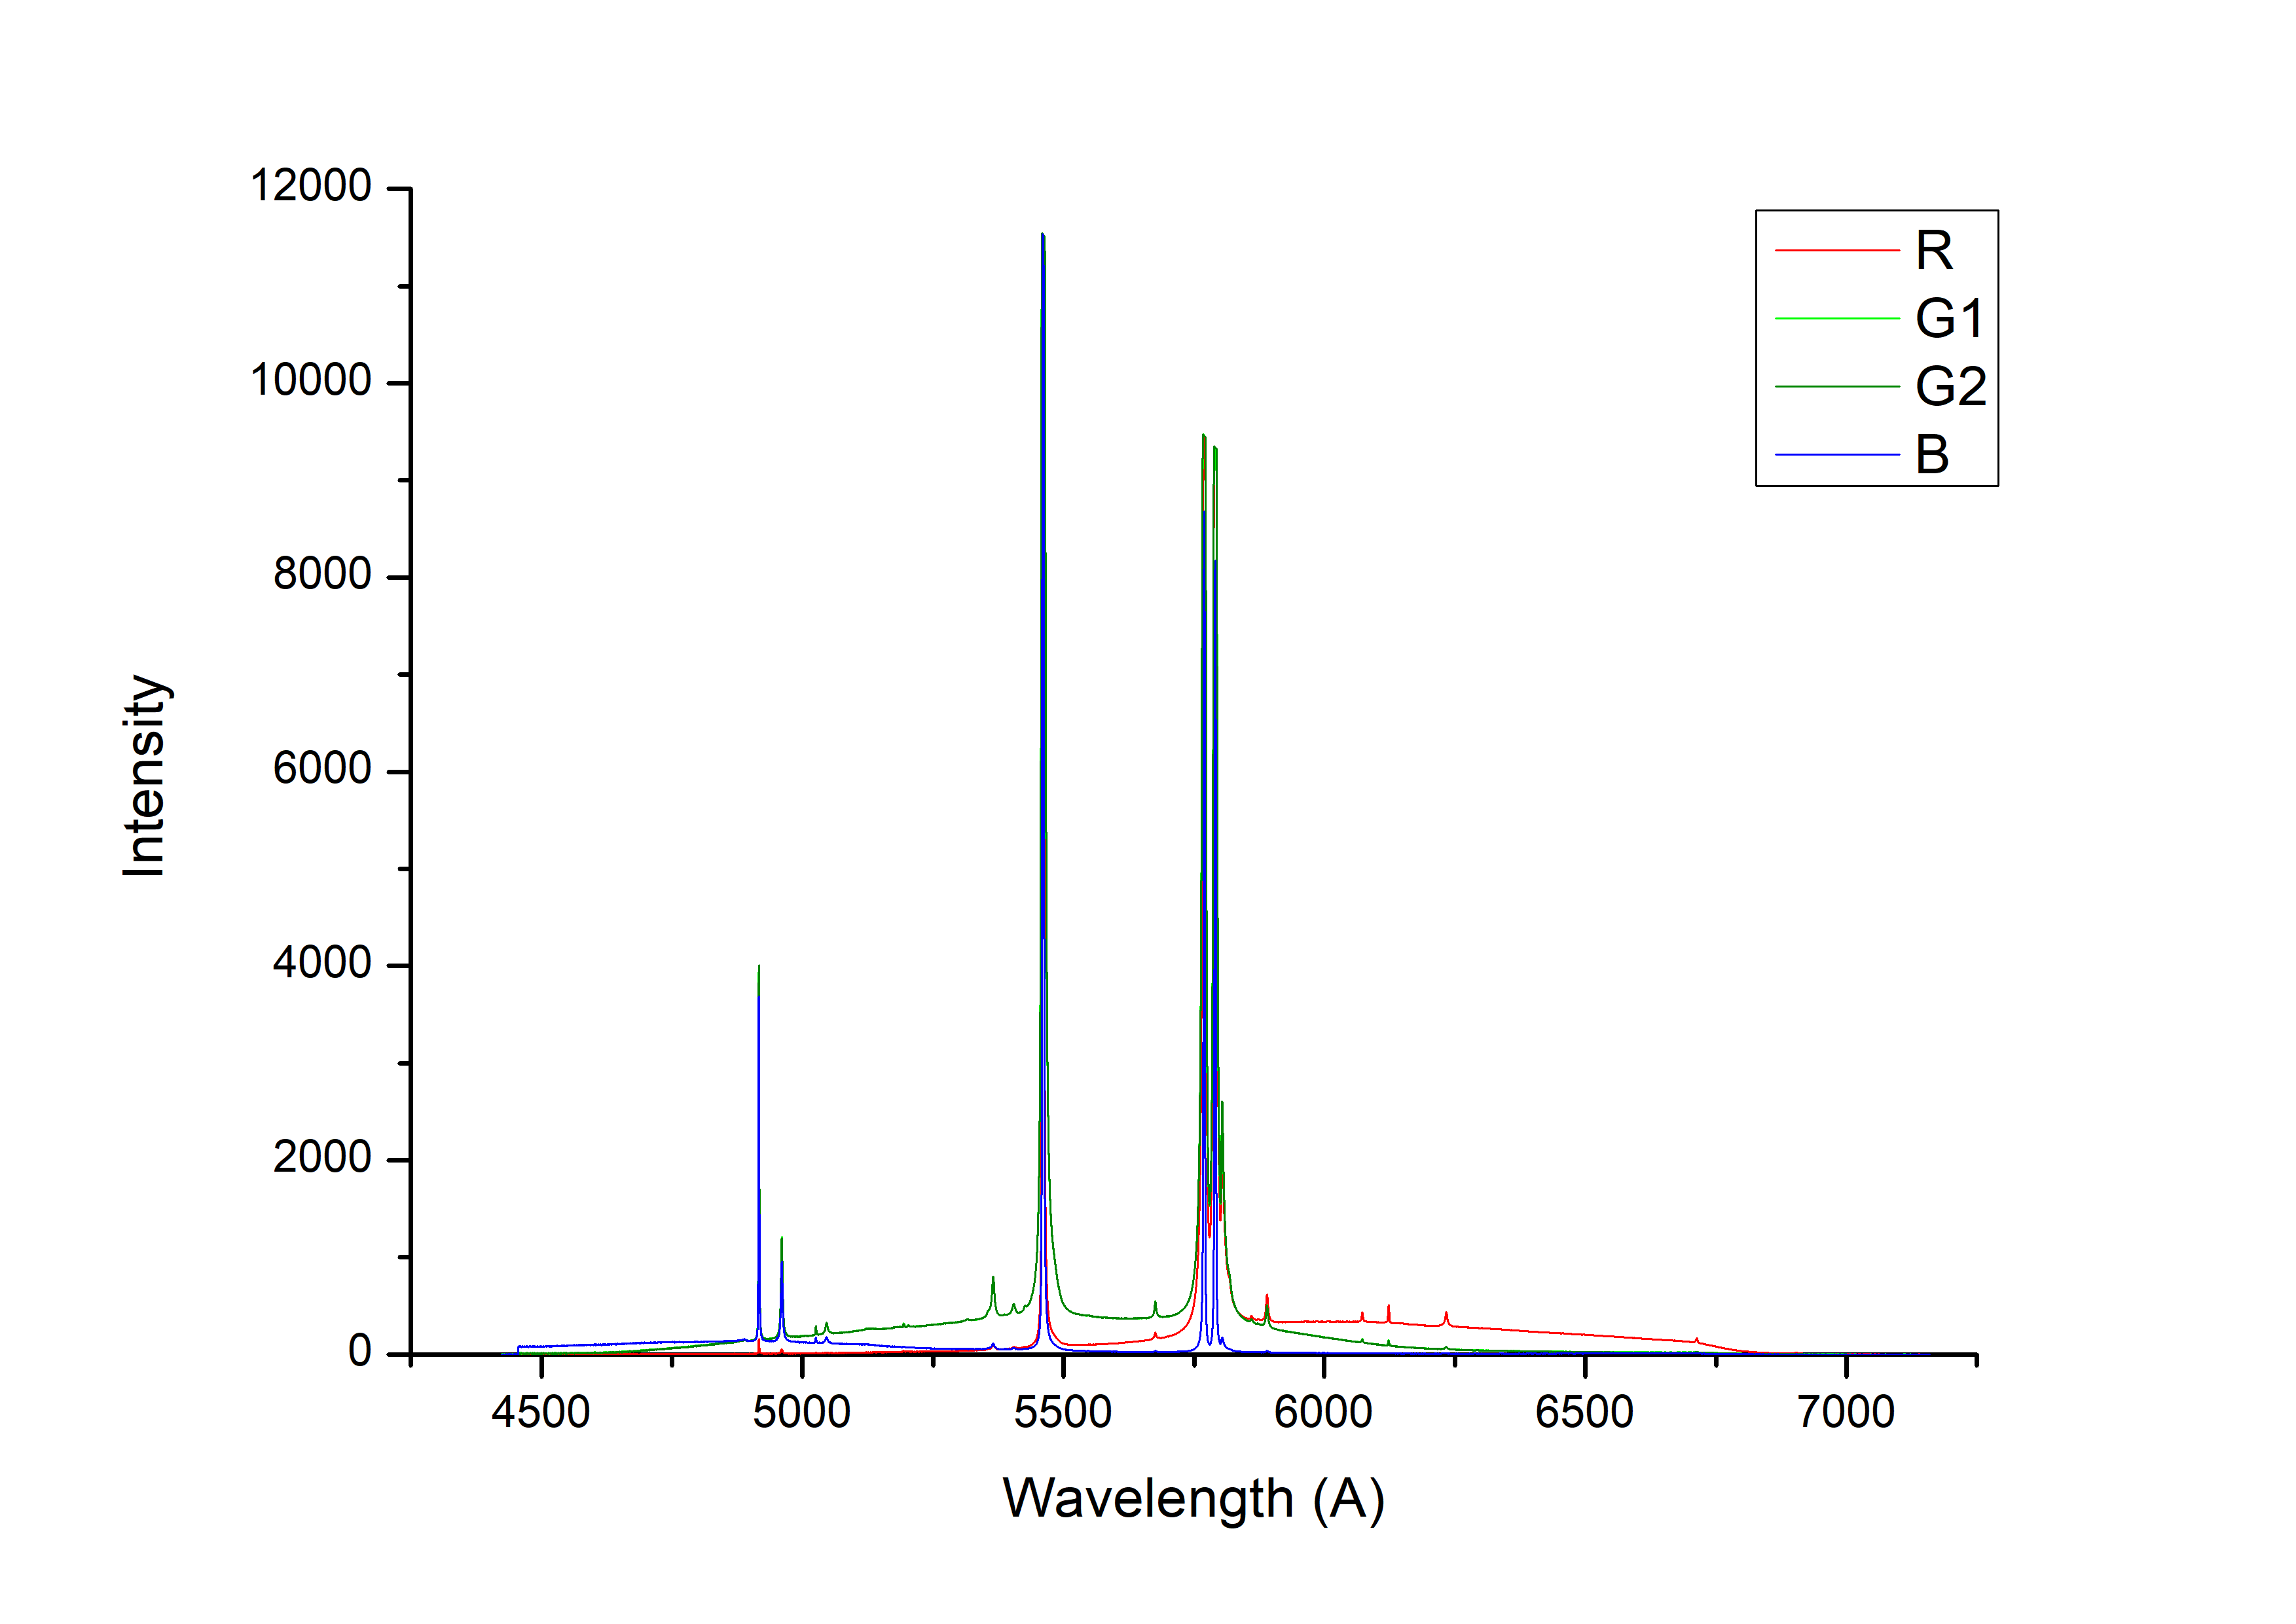
\includegraphics[width=\textwidth]{Graph2.png}
    \caption{График спектра ртутной лампы}
    \label{fig:vac}
\end{figure}

\begin{figure}[h]
    \centering
    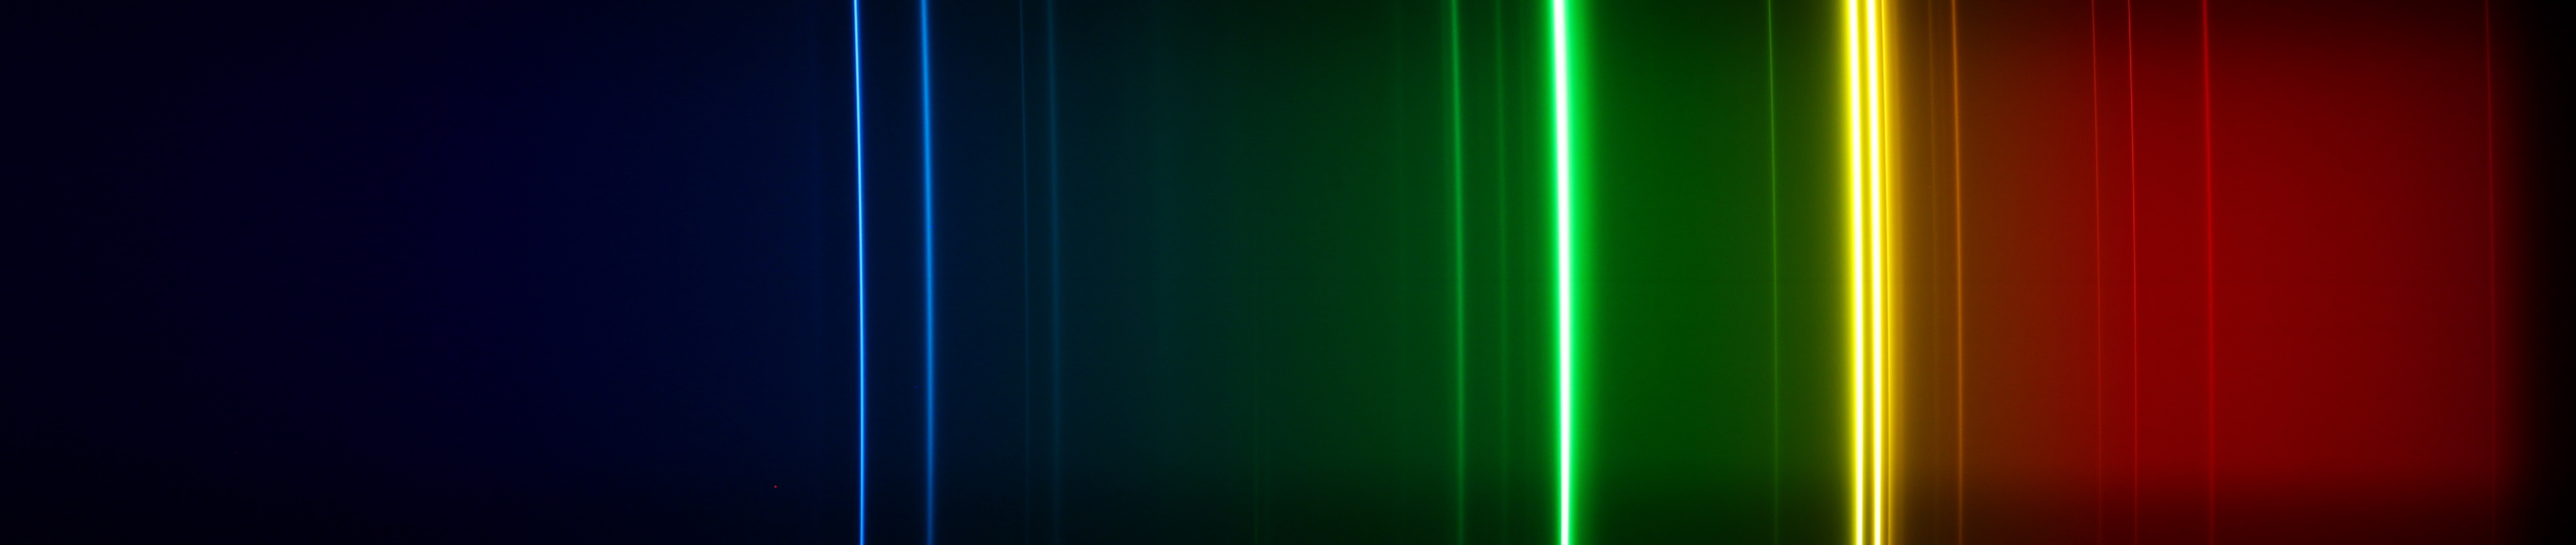
\includegraphics[width=15cm]{Hg_cut.JPG}
    \caption{Фотография спектра ртути}
    \label{fig:vac}
\end{figure}

\item Снимем спектр водородной лампы, представим его график на рис. 3, и фотографию на рис. 4. Измерим положение линий $H_{\alpha}$ и $H_{\beta}$ (линии в более коротковолновой области в спектр не попали):
\begin{center}
    $H_{\alpha} = 6563$ \AA \\
    $H_{\beta} = 4862$ \AA 
\end{center}


    \begin{figure}[h]
    \centering
    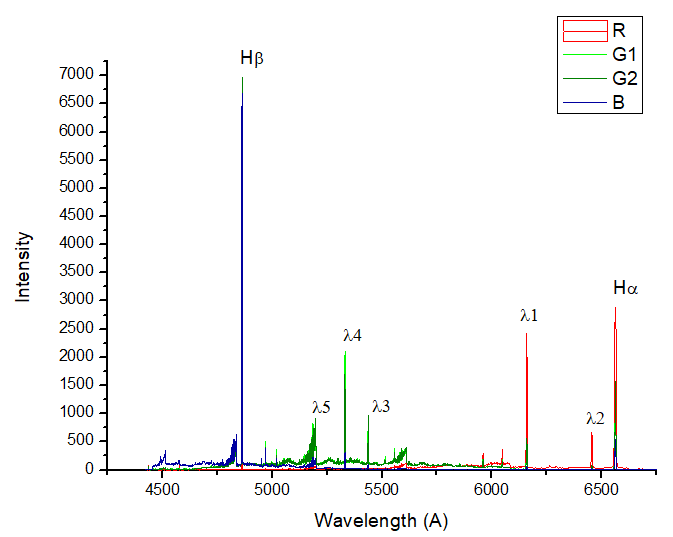
\includegraphics[width=\textwidth]{Graph2_1.PNG}
    \caption{График спектра водородной лампы}
    \label{fig:vac}
\end{figure}

\begin{figure}[h]
    \centering
    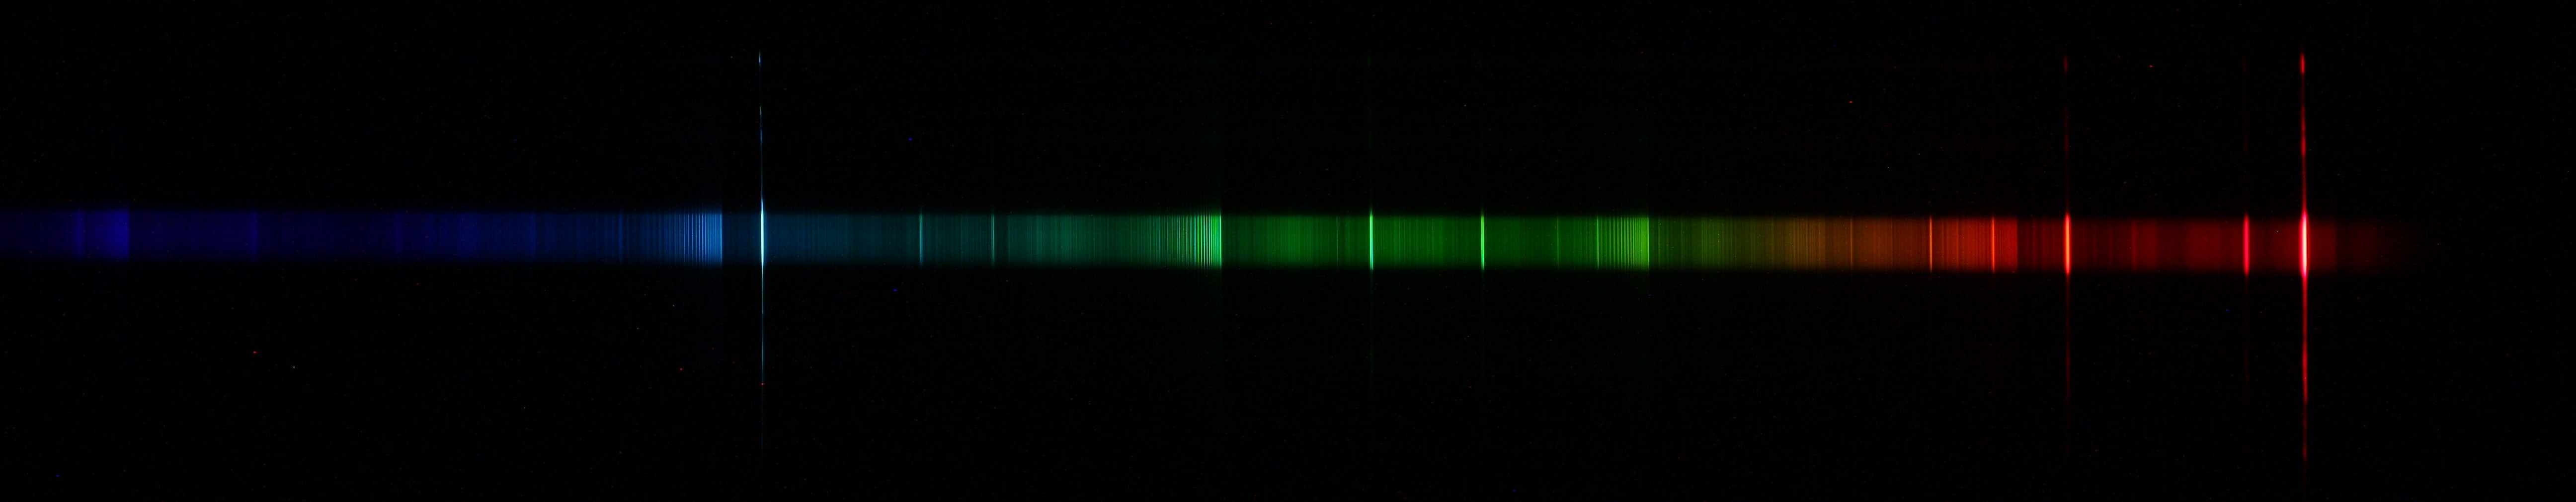
\includegraphics[width=15cm]{Hydrogene-cut.jpg}
    \caption{Фотография спектра водородной лампы}
    \label{fig:vac}
\end{figure}

\begin{figure}[h]
    \centering
    
\includegraphics[width=15cm]{Oxygen_spectrum_visible.png}
    \caption{Фотография спектра кислорода}
    \label{fig:vac}
\end{figure}

В спектре также присутствуют следующие достаточно сильные линии:
\begin{center}
    $\lambda_1 = 6158$ \AA - предположительно, кислород \\
    $\lambda_2 = 6456$ \AA - предположительно, кислород или ионизированный азот \\
    $\lambda_3 = 5437$ \AA - предположительно, кислород \\
    $\lambda_4 = 5331$ \AA - предположительно, кислород \\
    $\lambda_5 = 5200$ \AA - предположительно, кислород \\
\end{center}

\item По результатам измерения линий водорода определим постоянную Ридберга:
\begin{center}
    $Z = 1, n = 2, m = 3, \lambda_23 = 6563$ \AA \hspace{1cm} $R_{\alpha} = 109712.9$ см$^{-1}$ \\
    $Z = 1, n = 2, m = 4, \lambda_23 = 4862$ \AA \hspace{1cm} $R_{\beta} = 109694.2$ см$^{-1}$ \\
    Табличное значение: $R = 109737.3$ см$^{-1}$
\end{center}

\end{enumerate}

\clearpage

\section{Вывод}
В ходе работы были измерены следующие спектры:
\begin{itemize}
    \item калибровочный спектр ртутной лампы
    \item спектр водородной лампы
\end{itemize}

При измерении спектра ртутной лампы было обнаружено, что помимо водорода в лампе, предположительно, присутствует молекулярный кислород и/или азот. \par
Также в ходе работы было с высокой точностью измерено значение постоянной Ридберга для бесконечной массы: 
\begin{center}
    $R_{\alpha} = 109712.9$ см$^{-1}$ \\
    $R_{\beta} = 109694.2$ см$^{-1}$ \\
    Табличное значение: $R = 109737.3$ см$^{-1}$
\end{center}

\end{document}
